\picturechapterr{Introduction} \label{ch-1}

{
  \begin{center}
    \vspace*{0.5cm}
    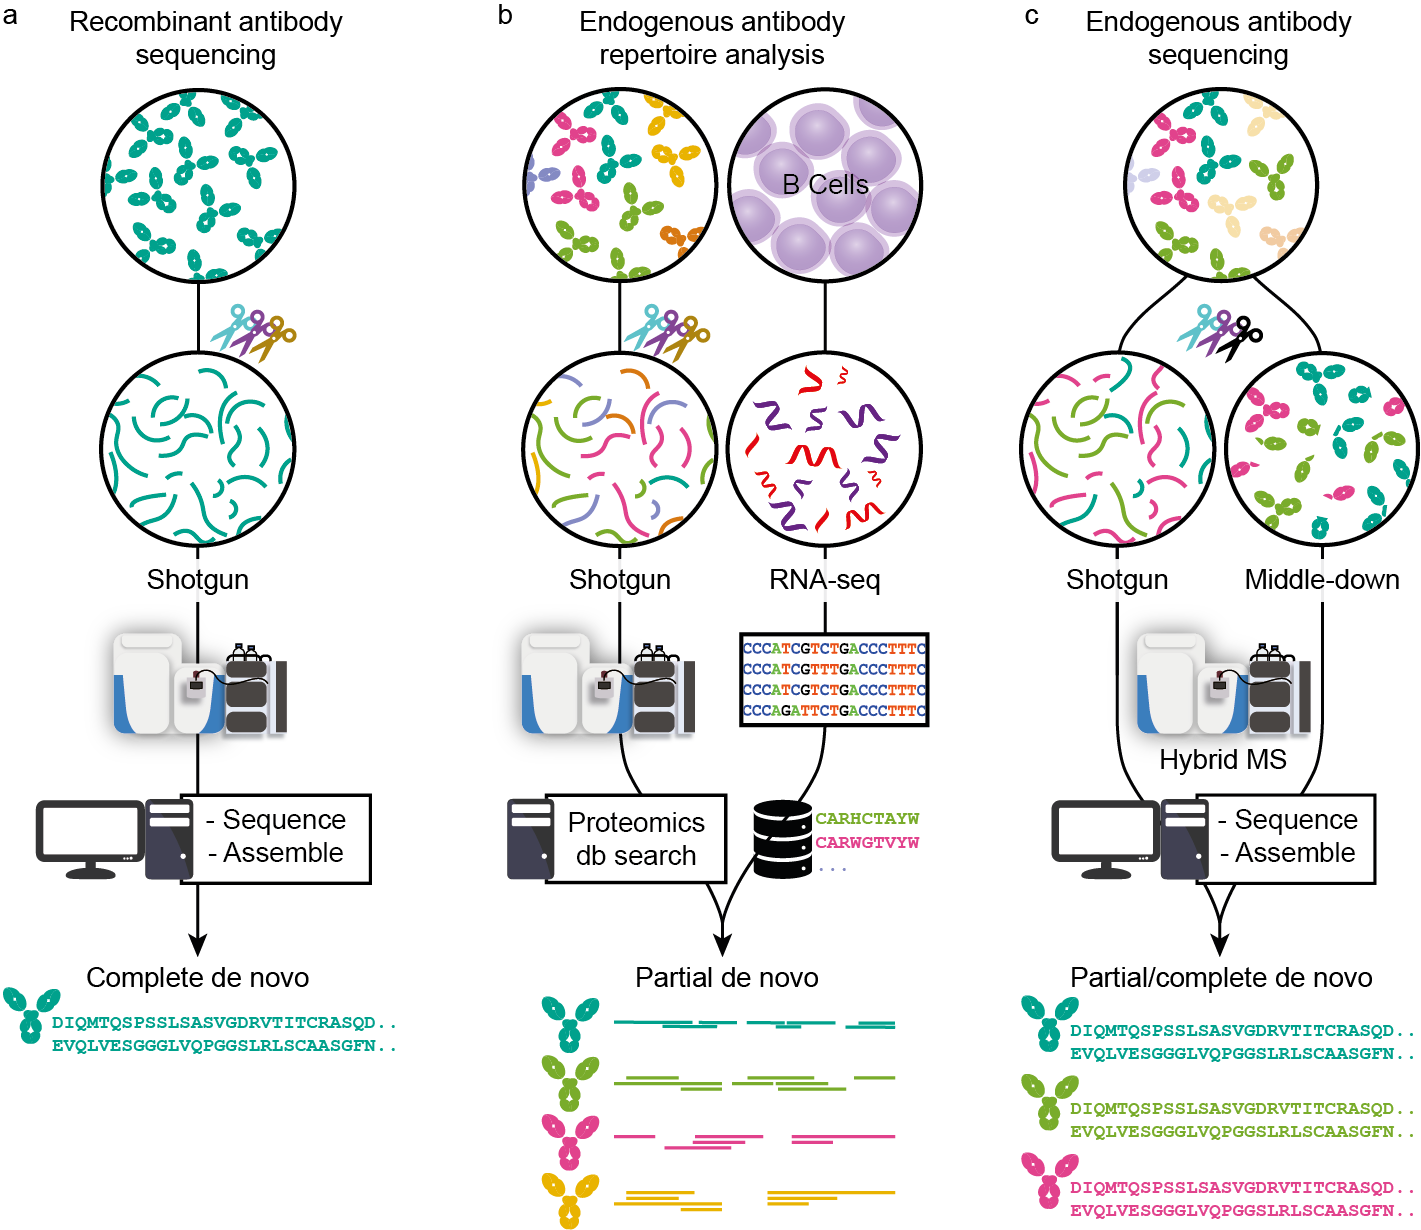
\includegraphics[]{Chapter.1/Figures/ch1.png}
    \vspace{0.25cm}
  \end{center}
}

\begin{flushleft}
  \vspace*{\fill}
  \rule{\textwidth}{1pt}\\[0cm]
  This chapter includes parts of the following publication:\\
  \textbf{A perspective towards mass-spectrometry-based \emph{de novo} sequencing of endogenous antibodies}\\
  \footnotesize
  \vspace{0.3cm}
  Sebastiaan C. de Graaf*, Max Hoek*, Sem Tamara and Albert J.R. Heck \\
  %%\vspace{0.3cm}
  \textbf{\emph{mAbs}} (2021), 14:1, 2079449, DOI: 10.1080/19420862.2022.2079449 \emph{Review}\\
  %%\footnotesize
  \vspace{0.3cm}
  \textsuperscript{*} These authors contributed equally to this work

\end{flushleft}
\newpage

\thumbforchapter

\section{Prelude - The importance of antibodies}
\lettrine[lraise=0.1, nindent=0em, slope=-.5em]{A}{round} the time of their initial discovery, antibodies were termed by various illustrious names, such as ‘Immunkörper’, ‘Amboceptor’, and ‘Zwischenkörper’, among many others. These terms were used more than a century ago to describe substances with antitoxin, lysin, agglutinin, and precipitin activities \cite{london1902der, lindenmann1984origin}. Nowadays, the generally accepted term \emph{antibody} refers to secreted immunoglobulins (Igs), whose sequence variety is several orders more diverse than the assortment of their historical names. Antibodies represent some of the most important molecules in the human immune system. Over the last century, Igs have been intensively studied because of their role in combatting infectious diseases and have taken centre stage for development of therapeutics in the last decade \cite{marks2020how, raybould2020thera-sabdab:, kaplon2021antibodies}. Beyond infectious diseases, recombinant antibodies are now also developed for cancer, rheumatoid arthritis, and various other pathological conditions \cite{singh2018monoclonal}. As key entities in the body’s defence mechanism, circulating antibodies are found in various bodily fluids, such as serum, saliva, milk, the lumen of the gut, and cerebrospinal fluid \cite{schroeder2010structure}. New leads for biotherapeutic development of recombinant antibodies come either from immunizing animals with specific antigens, or by discovering pathogen-neutralizing antibodies from recovered patients \cite{bornholdt2016isolation, corti2016protective, valgardsdottir2021identification}.
The estimated diversity of Ig molecules a human body can generate extends beyond 10\textsuperscript{15} theoretical sequences \cite{schroederjr.2006similarity, briney2019commonality}, indicating that each antigen may lead to a unique antibody response. These 10\textsuperscript{15} possible antibody sequences are all unique yet highly alike, posing a serious challenge for their characterization and sequencing, which has remained, to this day, a tremendously challenging task. Ideally, one would like to sequence antibodies at the protein level instead of through B-cell receptor (BCR) sequencing \cite{hom2022exploring}, as is currently the norm, to more directly probe circulating antibody repertoires and their relative abundances in specific environments. Mass spectrometry (MS) is expected to be the method of choice to potentially achieve this feat, as MS-based protein analysis has advanced and matured considerably \cite{altelaar2013next-generation, aebersold2016mass-spectrometric}. However, antibodies represent a very special and rather challenging class of proteins. Consequently, while MS has already been used to characterize and sequence highly purified monoclonal antibodies (mAbs) \cite{sen2017automated, peng2021mass, srzentić2020interlaboratory}, further technical developments in sample preparation and data analysis are needed to incorporate MS fully and efficiently into an endogenous humoral antibody discovery and characterization pipeline. In this thesis, I evaluate the role that MS can play in sequencing, identifying, and characterizing antibodies, focusing mainly on emerging strategies employed to enable identification and characterization of endogenous neutralizing antibodies.

\subsection{Nomenclature, structure, and diversity of antibodies}
Humoral human antibodies are complex proteins produced by B cells \cite{chiu2019antibody, schroeder2010structure}. Most antibody molecules (e.g. IgGs) are made up of four protein chains: two identical light chains and two identical heavy chains, which are interconnected by disulphide bridges (\textbf{\autoref{fig:fig1.1}}). The light and heavy chain form two heterodimers, which are connected via disulphide bridges in the hinge region to form the intact antibody. Functionally, the intact antibody can be divided into two antigen-binding domains (also known as Fab or fragment antigen-binding) and a constant domain (also known as Fc or fragment crystallizable) \cite{porter1959hydrolysis} (\textbf{\autoref{fig:fig1.1}a}). The Fc is the effector entity of the antibody and can bind to Fc-receptors on immune cells \cite{schroeder2010structure} and mediate immune effector responses such as phagocytosis, antibody-dependent cell-mediated cytotoxicity, respiratory burst, and cytokine release \cite{herr2003insights}. In contrast to the fully conserved sequence and structure of the Fc, the Fab is responsible for the vast diversity in recognized antigens and is thus hypervariable.
Because there is an endless and constantly evolving pool of pathogens, the antibody repertoire needs to be incredibly diverse and versatile to counteract these challenges \cite{charlesajaneway2001generation, alberts2002generation}. In humans, this enormous diversity in the potential antibody repertoire is achieved through several mechanisms. Starting at the genomic level, the light and heavy chains are encoded in four genes each: variable (V), diversity (D), joining (J), and constant (C), with the light chain lacking the D-gene. These genes are encoded in multiple alleles, which can recombine to a staggering number of combinations (\textbf{\autoref{fig:fig1.1}b}) \cite{jeske1984junctional}. The recombination process is also error-prone, leading to insertions and deletions at the junctions between the regions, referred to as junctional diversity. By recombination alone, the number of possible variable domain sequences already reaches tens of thousands. However, the eventual antibody diversity is expanded even further by natural polymorphisms, mutations, and class switching. As the major contributor to antibody hypervariability, somatic hypermutations can occur during B-cell affinity maturation and do so at a million-fold increased rate compared to the usual mutation rates \cite{schroederjr.2006similarity}. These mutations are largely concentrated in the complementarity-determining regions (CDR1-3), separated by framework regions (FR1-4), which form the conserved backbone of the Fab structure (\textbf{\autoref{fig:fig1.1}c}). Located at the tips of the Y-shaped antibody structure, CDRs are primarily responsible for antigen binding, and, therefore, elucidation of their sequences is of the utmost importance for antibody discovery.
\begin{figure*}[!htb]
  \center
  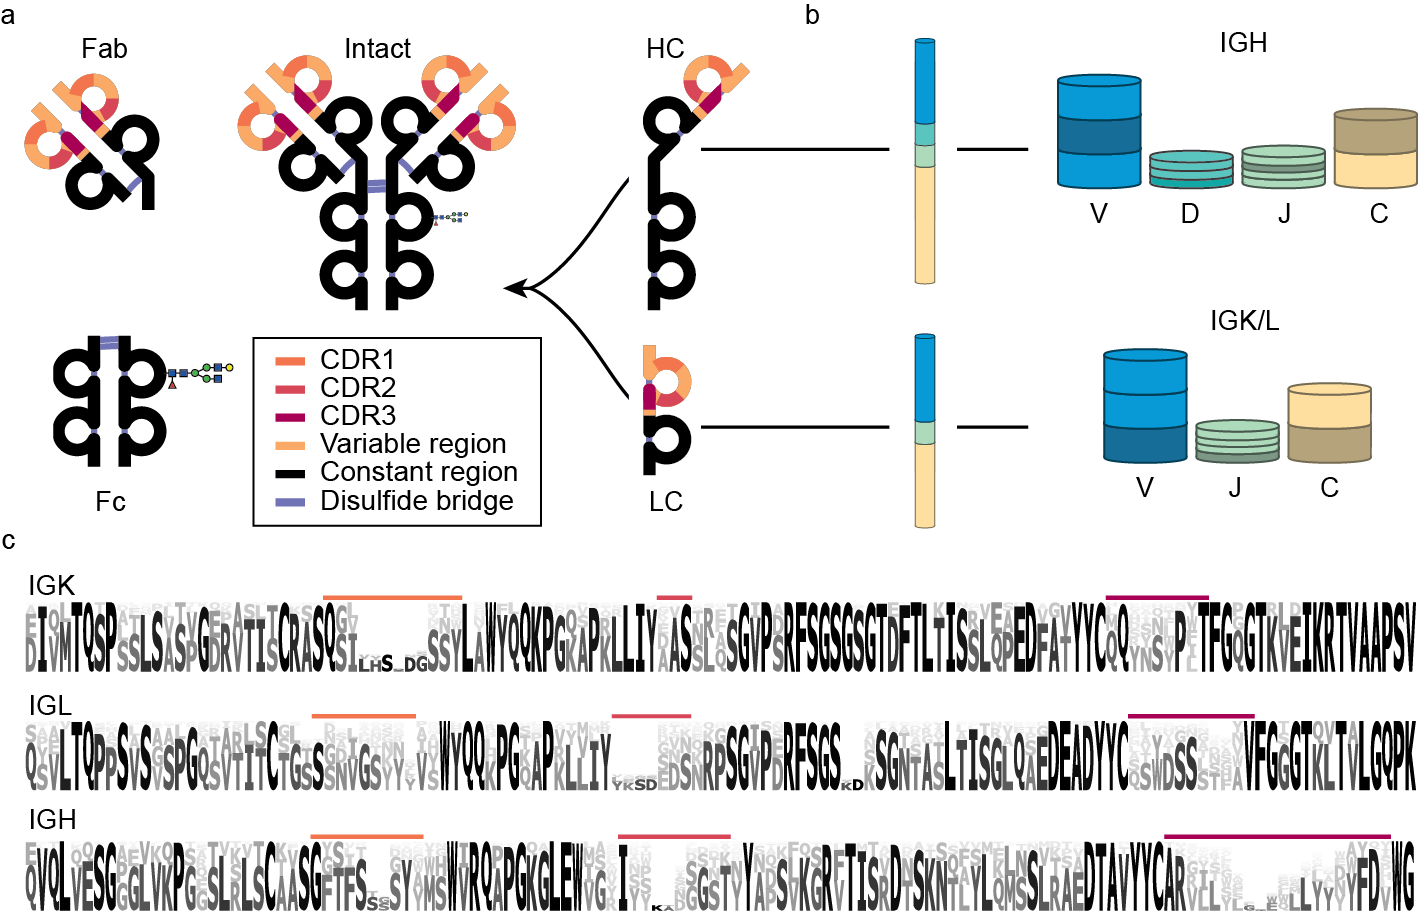
\includegraphics[]{Chapter.1/Figures/f1.png}
  \caption{
    \textbf{Nomenclature, structure, and diversity of IgG1 antibodies.}
    ~~a) Nomenclature and protein fragments of an IgG1 molecule. The antigen-binding domain, containing light and heavy chain (LC and HC respectively) variable regions, is termed Fab (or Fab2 when dimerized). The constant part of the heavy chain carrying an N-glycosylation site is called Fc. Other IgG subclasses vary in their heavy chain constant region (Fc) and disulphide patterns. ~~b) The diversity in antibodies originates primarily from the V, D, J, and C-allele (each annotated with a distinct colour) recombination process. In this process, each of many individual V, D, J, and C-alleles can recombine with any of the other gene segments, yielding thousands of possible combinations, in particular for the heavy chain, which incorporates the most diverse D region. ~~c) Sequence logo created by the alignment of in silico generated sequences of Ig kappa (IGK) and lambda (IGL) light chains and Ig heavy chain (IGH) from the international ImMunoGeneTics (IMGT) information system database \cite{lefranc2003imgt}. Even though the displayed sequences are part of the variable domain, large stretches of these sequences, also known as the framework regions (FRs), are relatively conserved, compared to the hypervariable complementarity determining regions (CDRs), coloured in accordance with ~~a) .
  }
  \label{fig:fig1.1}
\end{figure*}
The Fc part of Igs is used to classify antibodies into one of 5 classes: IgA, IgD, IgE, IgG, and IgM. Some of these classes are divided further into subclasses denoted by numbers, e.g., IgG1-4 or IgA1 and IgA2. Although the function of the classes and subclasses is different, their variable regions stem from the shared pool of genes. Therefore, for simplicity, in this review, we focus primarily on IgG1, the most abundant antibody subclass in serum, and the predominantly used subclass for biotherapeutic development. Still, concerning \emph{de novo} sequencing by MS, different Ig classes and subclasses pose similar challenges and opportunities.

\subsection{Modalities of MS-based antibody analysis}
Proteomics is the large-scale study of proteins. Many different peptide- and protein-centric MS-based approaches have been developed for proteomics, whereby some of these have been adapted for \emph{de novo} sequence analysis of antibodies.
Bottom-up (BU) or shotgun proteomics is by far the most widespread approach in MS-based protein analysis. In it, protein samples are digested by one or more proteases, and the resulting peptides are separated by some form of liquid chromatography (usually reversed-phase (RP)-HPLC), after which their peptide masses are recorded (MS1). Highly abundant precursor ions are then selected for fragmentation, and the masses of their fragment ions (MS2) are recorded.
Because digestion and MS-based fragmentation adhere to highly specific rules, peptides and their gas-phase fragment ions can be predicted. Consequently, peptides and their parent proteins are identified by comparing recorded spectra to the spectra simulated from protein or DNA databases \cite{aebersold2003mass}. For antibody sequencing, personalized databases are required for identification. Yet, digestion-based strategies are still widely used even without an available database. Individual spectra can be \emph{de novo} sequenced, and the resulting reads can be assembled into full-length sequences \cite{tran2016complete, guthals2012shotgun, sen2017automated}.
Additionally, intact mass analysis is a useful tool for protein analysis, providing masses that can be considered fingerprints of the species (known as proteoforms) present in the sample. Comparing different masses can lead to conclusions about relations between multiple species, for instance, if they differ by the mass of a known mutation, post-translational modification (PTM), or signal peptide \cite{donnelly2019best}. In the case of antibodies, such analysis can be performed with the protein in its native, and possibly complexed, state, or unfolded and separated into the comprising chains. Such approaches can provide valuable insights in the context of antibodies, e.g., by assessing the complexity of antibody repertoire or following changes in abundance of specific clones \cite{bondt2021human}. When applied to \emph{de novo} sequencing, the precursor mass knowledge can help determining the light and heavy chain pairing or sequence prediction accuracy in BU sequencing \cite{guthals2017de}.
In addition, both denatured and native antibodies can also be fragmented to yield some sequence information, this approach is called top-down (TD) MS. Because of the much larger size and higher charge of the analysed species, such intact-protein fragmentation spectra are more complex and harder to interpret than peptide spectra \cite{toby2016progress, compton2011on}. To mitigate this, specific proteases can be used to cleave proteins into smaller subunits. This practice is called middle-down (MD) MS, and in the context of antibodies it is often performed by cleaving the hinge region of the heavy chain before MS analysis \cite{johansson2008ides:}. Fragmentation spectra of entire chains or intact antibodies can provide valuable tools for both sequence determination and validation of sequence predictions, as fragmentation is highly specific for the precursor clone, which is often untrue in BU analysis \cite{fornelli2014middle-down}.

\section{The emerging role of mass spectrometry in antibody discovery}
Due to the structural complexity and immense sequence diversity of antibodies, the development of therapeutic antibodies has always been a very challenging and labour-intense task, especially when compared to small-molecule drug development. For example, the discovery of Trastuzumab was achieved by using mice immunized with antigen-expressing cells. Following the generation and selection of hybridomas that showed specific activity \cite{hudziak1989p}, the sequence of the selected antibody was determined after cloning and expression. A humanized antibody could be produced only thereafter by adapting and modifying the sequence accordingly \cite{carter1992humanization}. The same approach was used in the development of several other mAbs \cite{tsurushita2005design, khoja2015pembrolizumab, busse2001omalizumab, presta1993humanization}. Apart from being expensive and laborious, these early strategies required knowledge and availability of purified antigens and animal models that can produce specific antibodies in response to these antigens \cite{lu2020development}.
More recently, alternative strategies for antibody discovery have been explored starting with the screening of B cells from individuals who successfully overcame an infection. In this approach, peripheral blood mononuclear cells (PBMCs) are isolated, immortalized, and screened for antigen reactivity. The reactive clones are further expanded and characterized. This method has proven effective in finding new neutralizing antibodies that can be used to combat certain infectious diseases, e.g. Ebola \cite{bornholdt2016isolation, corti2016protective} or severe acute respiratory syndrome coronavirus 2 (SARS-CoV-2) \cite{valgardsdottir2021identification}. These recent advances show that the discovery of antibodies from human subjects, in addition to animal models, represents a viable method for developing new avenues for therapies. However, it may be even more advantageous to discover and characterize mature antibody clones directly from clinical samples at the protein level in their functionally matured and active form.
\begin{figure*}[!htb]
  \center
  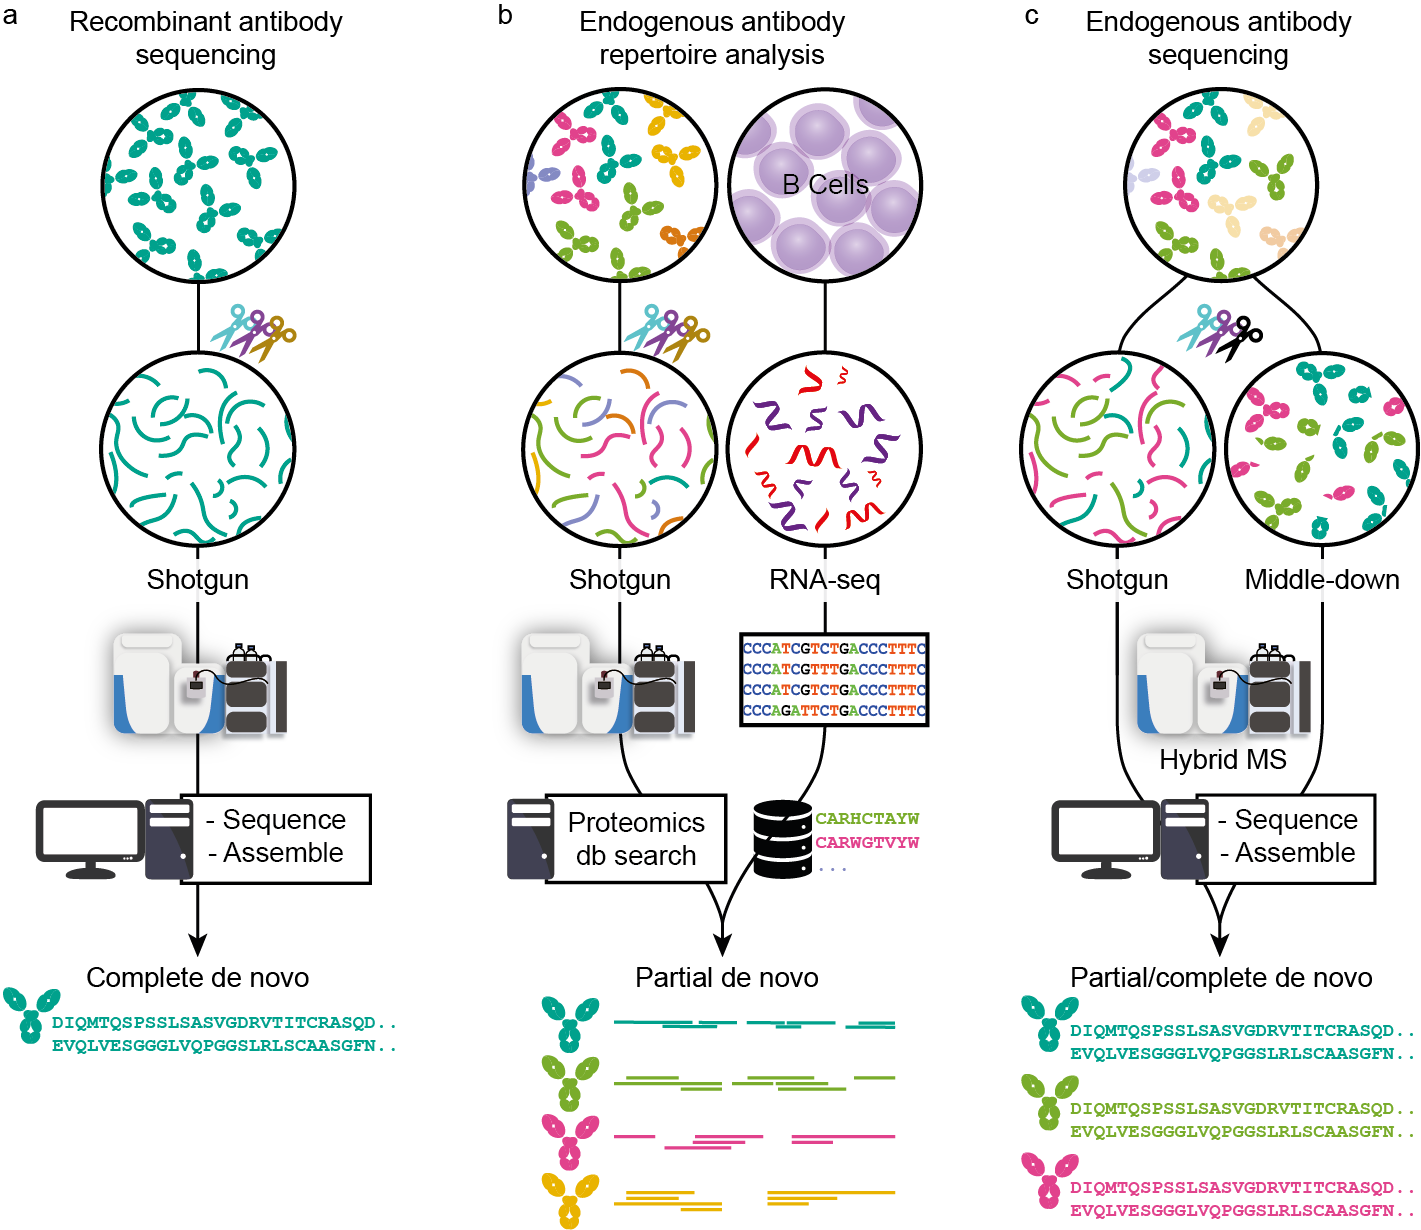
\includegraphics[]{Chapter.1/Figures/f2.png}
  \caption{
    \textbf{Three approaches in MS-based antibody sequencing.}
    ~~a) Recombinant antibody sequencing generally starts with abundant highly purified mAbs, which can be fully sequenced through BU MS, where hundreds of peptides are generated by digesting the mAb with one or several proteases, providing multiple overlapping short sequence reads. After liquid chromatography-mass spectrometry (LC-MS) measurement, the spectra can be processed by several different \emph{de novo} sequencing software solutions and assembled into full-length mAb sequences \cite{peng2021mass}. ~~b) In repertoire analysis, a sequence database is generated through B-cell sequencing, and MS-data is obtained through BU MS experiments. After generation of the personalized database, a high throughput of the LC-MS is possible \cite{georgiou2014promise}. While not strictly \emph{de novo} since only hits from the sequence database are identified, it is a powerful tool for antibody repertoire analysis. ~~c) Endogenous antibody sequencing cannot rely on BU MS alone, as direct sequencing of endogenous humoral antibodies is hampered by inherent challenges and complexity. Emerging MD and TD MS techniques provide clone-specific sequence information highly complementary to traditional sequencing. Integrating BU MS and MD/TD MS makes it possible to achieve full-length coverage of antibody sequences \cite{bondt2021human}.
  }
  \label{fig:fig1.2}
\end{figure*}

In recent years, MS-based proteomics has advanced tremendously in sample preparation, MS and liquid chromatography instrumentation, and data analysis \cite{altelaar2013next-generation, aebersold2016mass-spectrometric}. Using all these advances, antibody sequencing at the protein level by MS has come within reach. \textbf{\autoref{fig:fig1.2}} highlights three – chiefly MS-based – strategies used to determine antibody sequences. These three pillars are primarily classified by the source of sample material and the attainable sequencing information. The first strategy applies to highly purified recombinant antibodies that are now amenable for full sequencing with BU MS, often by combining several different proteases and advanced algorithms. Second, hybrid approaches have been introduced for analysing endogenous antibody repertoires by combining MS-based techniques with genomics or transcriptomics, e.g., whole genome sequencing or BCR sequencing, ideally from the same donor. The third set of techniques encompasses several MS-based \emph{de novo} approaches that aim to determine complete antibody sequences of selected clones directly from clinical samples without the aid from alternative omics data. While each strategy is distinct, they all share common aspects.


\subsection{MS-based sequencing of monoclonal antibodies}
Before delving into the topic of MS-based sequencing of endogenous antibodies from clinical samples, we first discuss the current state-of-the-art sequencing approaches developed for recombinant mAbs. Principles of mAb sequencing by MS share many technical considerations with sequencing of antibodies present in complex mixtures. Furthermore, currently available strategies for recombinant mAb sequencing provide great context for discussing limitations and bottlenecks that hamper sequencing of endogenous antibody clones.

\subsubsection{Shotgun, bottom-up strategies used for sequencing of highly purified mAbs}
Antibodies are often analysed after digestion with one or more proteases to generate peptides (\textbf{\autoref{fig:fig1.2}}). Such peptide-centric approaches are known as BU MS and represent the most popular type of proteomics experiments. In contrast to most shotgun proteomics experiments, \emph{de novo} sequencing through BU MS necessitates a high depth of sequence coverage, i.e. each sequence position in the antibody is ideally supported by multiple overlapping unique peptides. With a typical highly specific protease such as trypsin, which cleaves C-terminally of lysine and arginine, and a low number of missed cleavages, sequence-coverage depth is often limited because only a few of the generated peptides overlap in sequence. Although this suits standard shotgun proteomics experiments, which do not require full sequence coverage of the analysed proteins, \emph{de novo} sequencing of antibodies thus requires other approaches.
Several methods to generate complete and deep sequence coverage by overlapping peptides have been introduced. For example, a shortened protease incubation time was successfully used to increase the number of peptides carrying missed cleavage sites \cite{morsa2019multi-enzymatic}. Some proteases generate a high number of overlapping peptides through non-specific cleavage \cite{bandeira2008beyond, castellana2010template, guthals2017de}. Alternatively, non-specific cleavage can be also achieved through non-enzymatic treatment, e.g., microwave-assisted hydrolysis \cite{savidor2017database-independent}. For these methods to work, digestion conditions must be tightly controlled to avoid abnormally long or short peptides and ensure reproducibility. Another elegant option is to use multiple proteases with synergistic sequence specificities. For instance, Peng et al. \cite{peng2021mass} recently used a total of 9 proteases, both specific and non-specific, to successfully \emph{de novo} sequence a full-length anti-FLAG-M2 mouse mAb (\textbf{\autoref{fig:fig1.3}}). The strength of a large panel of proteases is shown in the validation of the CDR sequences by high scoring peptides covering the entire CDR. The 6 chosen peptides are the result of digestion by 5 different proteases (trypsin, chymotrypsin, lysC, thermolysin, and elastase, \textbf{\autoref{fig:fig1.3}a and b}).
Nowadays, most \emph{de novo} sequencing solutions, such as ALPS/PeaksAB \cite{tran2016complete}, GenoMS \cite{castellana2010template}, SuperNovo \cite{sen2017automated} and Champs \cite{liu2009automated} are quite successful in obtaining full sequence coverage of highly purified antibodies. To determine the antibody sequences \emph{de novo}, all these software tools require large number of overlapping peptides, spanning the entire sequence, which are successfully fragmented and converted into predicted peptide sequence reads (\textbf{\autoref{fig:fig1.2}a}). This necessitates generation of BU MS data by using multiple proteases. While complicating sample preparation and increasing the required amount, such multi-protease approaches are advantageous for \emph{de novo} sequencing by alleviating the sequence assembly problem.
\begin{figure*}[!htb]
  \center
  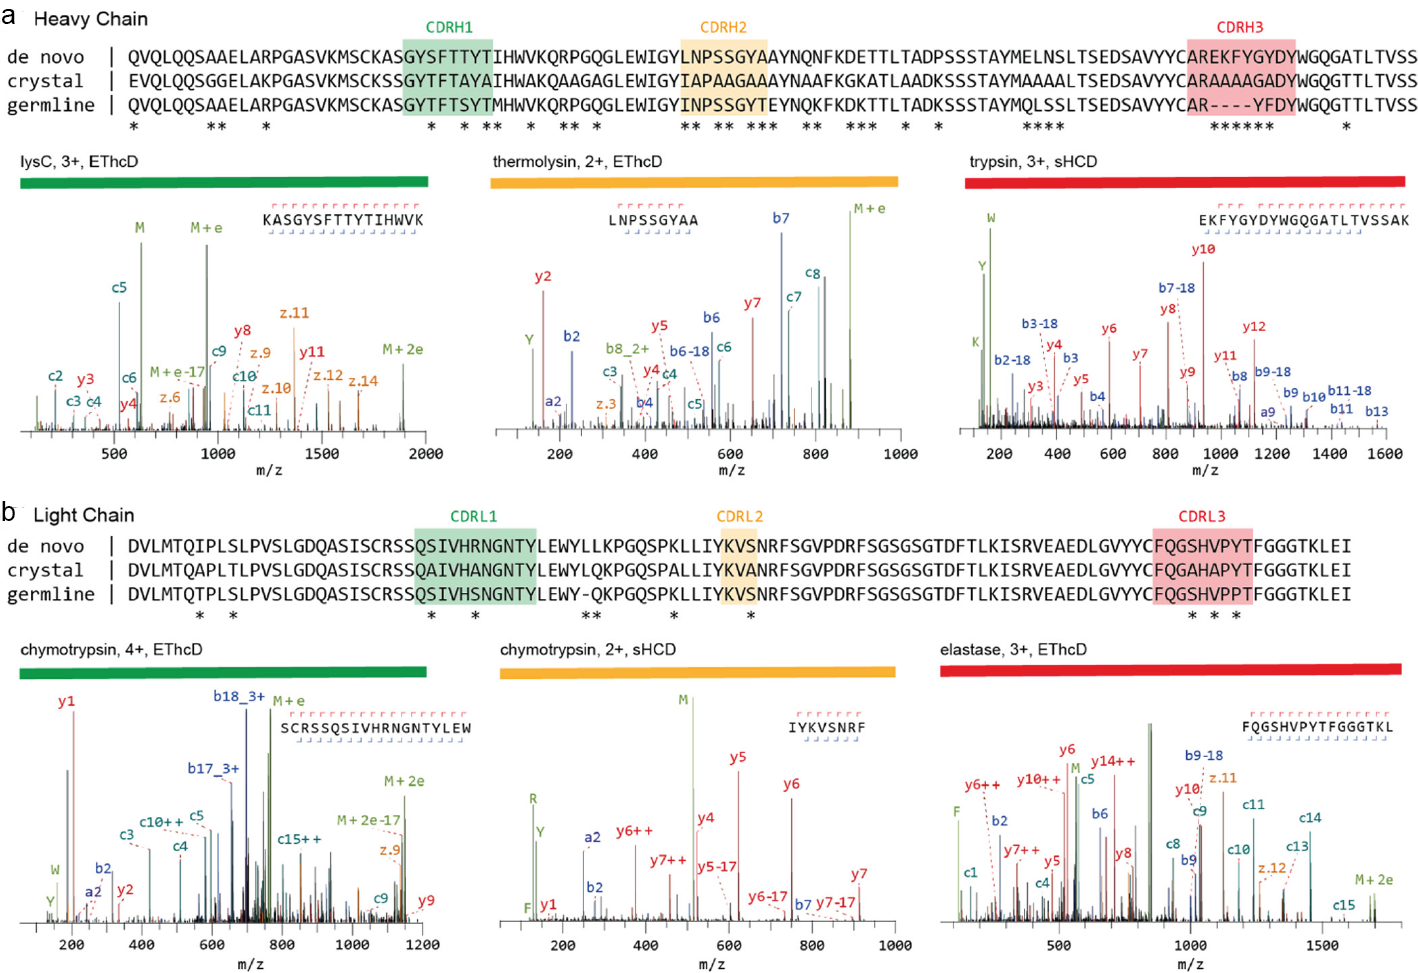
\includegraphics[]{Chapter.1/Figures/f3.png}
  \caption{
    \textbf{Sequencing of a monoclonal Anti-FLAG M2 antibody.} The variable regions of the heavy ~~a) and light chains ~~b) are shown. The \emph{de novo} sequence derived by MS is shown on top, alongside the previously published sequence used in the crystal structure of the Fab (PDB ID: 2G60), and germline sequence (IMGT-DomainGapAlign; IGHV1-04/IGHJ2; IGKV1-11$\star$7/IGKJ1). Differential residues are highlighted by asterisks (*). Exemplary MS/MS spectra in support of the assigned sequences are shown below the alignments, labelled with protease, precursor charge state, and fragmentation type. The peptide sequence and fragment coverage are indicated in the top-right of each spectrum spectra, with \emph{b/c} ions indicated in blue/teal and \emph{y/z} ions in red/orange. The same colour annotation is used for peaks in the spectra, with additional peaks such as intact/charge reduced precursors, neutral losses, and immonium ions indicated in green. To prevent overlapping peak labels, only a subset of successfully matched peaks are annotated. Figure and caption adapted from Peng et al. \cite{peng2021mass}
  }
  \label{fig:fig1.3}
\end{figure*}


\subsubsection{Benefits of complementary peptide fragmentation techniques}
In MS-based sequencing, extensive fragmentation of peptide ions is essential to generate arrays of adjacent fragments that reveal the amino acid sequence, often referred to as ion ladders or sequence tags (\textbf{\autoref{fig:fig1.4}a}). The amino acid sequence of the fragmented peptide is derived by comparing the mass difference between two adjacent fragment ion peaks to the masses of amino acids and combinations thereof. The produced fragment ion series must contain very few gaps larger than a single amino acid residue, because such gaps lead to exponential growth of the amino acid combinations that fit the mass difference, particularly for spectra of lower resolution \cite{he2018protein}. Since there is no universal fragmentation method that can produce uninterrupted fragment ion ladders for all possible peptides, it is highly advantageous to use various fragmentation methods with distinct mechanisms and specificities to complement each other (\textbf{\autoref{fig:fig1.4}b}) \cite{macias2020ion}. While collisional dissociation (CID/CAD/HCD) is the most used technique in shotgun proteomics experiments, multiple alternative fragmentation techniques have been introduced and have proven to be complementary. These specificities stem from the unique ion activation mechanisms employed by each method. In collision-based techniques, energy is deposited to the multiply protonated peptide ions through low-energetic collisions with inert neutral atoms or gas molecules. This energy is redistributed vibrationally throughout the peptide backbone, fragmenting the most labile bonds and yielding \emph{b/y}-type fragment ions, as defined by the Roepstorff-Fohlmann-Biemann ion nomenclature (\textbf{\autoref{fig:fig1.4}c}) \cite{roepstorff1984proposal}. Although protonated amide bonds are usually the most susceptible to fragmentation, collisional dissociation often also leads to loss of labile PTMs, such as phosphorylation and sialyation.
\begin{figure*}[!htb]
  \center
  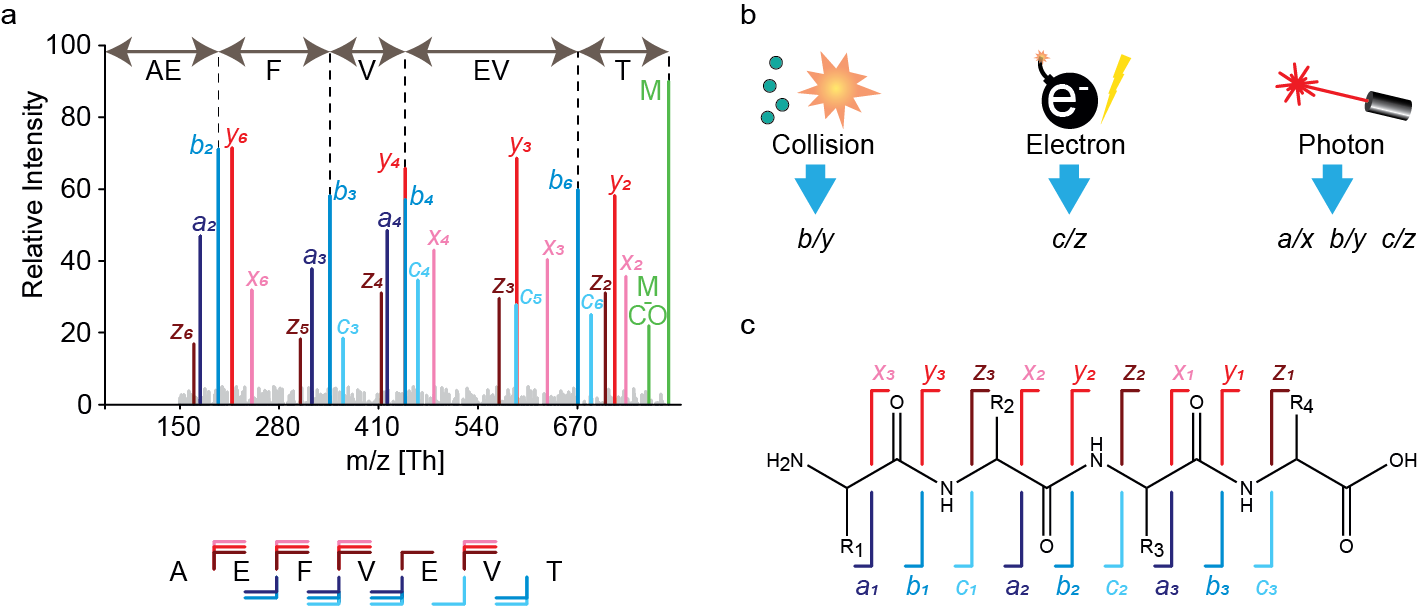
\includegraphics[]{Chapter.1/Figures/f4.png}
  \caption{
    \textbf{Peptide fragmentation in MS-based \emph{de novo} sequencing.} ~~a) An illustrative fragmentation spectrum. In the spectrum, fragment ion peaks are colour annotated according to the type of fragment ion (\emph{a}: purple, \emph{b}: blue, \emph{c}: light blue, \emph{x}: pink, \emph{y}: red, and \emph{z}: brown) the unfragmented peptide (precursor ion) is shown in green as well as the precursor ion with neutral loss of CO. Adjacent fragment ions of the same type have a mass difference corresponding to a single amino acid, which is used to determine the sequence as is illustrated for \emph{b}-ions above spectrum. Below the spectrum the amino acid sequence is shown together with the fragment ion annotation, N-terminal fragments (\emph{a-, b- ,c-}) are below the sequence and C-terminal fragments (\emph{x-, y-, z-}) are shown above the sequence. ~~b) Three predominant gas phase fragmentation techniques with their predominantly produced fragment ion types. Collisional dissociation (CID/CAD/HCD) predominantly yield \emph{b/y} ions. Electron based dissociation (ECD/ETD) yields \emph{c/z} ions. Contrary the other techniques, high energy photon based dissociation (UVPD) results in all fragment ion types \cite{brodbelt2016ion}. ~~c) The Roepstorff-Fohlmann-Biemann nomenclature used for peptide fragment ions denotes different fragment ion types by italic letters \emph{a-c} and \emph{x-z}. The numbering indicates the position of the bond in the amino acid sequence with respect to the N- and C-termini.
  }
  \label{fig:fig1.4}
\end{figure*}
In electron-based techniques (ECD/ETD), positively-charged peptide ions capture electrons, leading to the generation of odd-electron species that dissociate promptly without significant vibrational redistribution \cite{syka2004peptide, zubarev2000electron, mcluckey1998ion/ion}. In contrast to collisional dissociation, this process is not directed towards the most labile bonds, and produces distinctively \emph{c} and \emph{z} fragment ions through the dissociation of N-Cα bond (\textbf{\autoref{fig:fig1.4}c}). Similarly, high-energy photon-based activation techniques (UVPD) also cause bond dissociation without substantial energy redistribution. This is enabled by a number of chromophores along the peptide backbone and results in a wide array of co-occurring fragment ion types (\emph{a/x, b/y, c/z}), depending on the wavelength used \cite{brodbelt2016ion, brodbelt2020ultraviolet}. Highly energetic fragmentation methods can also lead to \emph{w}-type ions, which involve an amino acid side chain dissociation \cite{xiao2016distinguishing, kjeldsen2003distinguishing}. In \emph{de novo} sequencing, this may be advantageous since it allows to distinguish between leucine and isoleucine, which are commonly misassigned because they have an identical mass.
While having multiple fragment ion types in a single spectrum can complicate ion ladder detection (\textbf{\autoref{fig:fig1.4}a}), it can also provide insight into the direction of fragment ion series, revealing to which terminus (N or C) peptide fragments belong. This is possible due to the characteristic mass shift patterns of consecutive \emph{a, b, c} fragments and consecutive \emph{x, y, z} fragments originating from the same peptide bond. Horn et al. \cite{horn2000automated} pioneered this approach for \emph{de novo} protein sequencing by combining CID and ECD to discern between the N- and C-terminal fragment ions, which simplified the detection of consecutive fragment ions. Subsequently, many others have used similar strategies \cite{guthals2013sequencing-grade, vyatkina2017de, datta2009spectrum, horton2017comprehensive, bertsch2009de}.
The previously described publication by Peng et al. \cite{peng2021mass} also demonstrates the successful application of using multiple fragmentation techniques. They recorded spectra using a dual fragmentation scheme of both high-energy collision dissociation (HCD) and electron-transfer high-energy collision dissociation (EThcD), resulting in a reduced number of sequencing errors when compared to using a single fragmentation method. The spectra selected to support the CDR predictions are also derived from both fragmentation techniques, showing that this versatile fragmentation strategy can benefit sequence coverage in these challenging and important regions (\textbf{\autoref{fig:fig1.3}}).
Such multiplexing MS strategies have made \emph{de novo} sequencing of mAbs feasible, at least when they are of sufficient purity. However, the procedure is quite laborious as it often involves using multiple proteases to generate overlapping peptides and multiple peptide fragmentation techniques to obtain unambiguous sequence reads, which entails longer sample preparation time, the requirement of larger sample amounts, and extensive data acquisition.

\subsubsection{Homology-aided \emph{de novo} sequencing of antibodies}
To identify peptides and proteins, shotgun proteomics experiments rely on matching observed fragmentation spectra to theoretical spectra generated from sequence databases. However, complete and accurate mature sequences are not generally available for many proteins, especially for highly variable or frequently mutated proteins like antibodies. Instead, homologous sequences, primarily derived from genomic or transcriptomic experiments, can be used. For antibodies, the genes encoding for each of the regions (V, D, J, and C) are available as germline sequences and can be retrieved from the IMGT database \cite{lefranc2003imgt, lefranc2020immunoglobulins}. While such a database of homologous sequences can facilitate verification or guide predictions of \emph{de novo} sequences, it should be noted that the exact match to the target sequence is likely not present even in the most extensive databases. Traditional database searches are thus not applicable because they require exact mass matching of fragments, and a single amino acid mutation can prevent identification. Instead, error-tolerant fragment matching algorithms, either based on sequence alignments or subsequence (i.e., sequence tag) extractions, can use homologous databases to score experimentally determined sequences.
An example of a homology-aided approach is searching BU MS data from a sample of human antibodies against a proteome database such as Swiss-Prot, whereafter the identified peptides are aligned to the IMGT database \cite{schmelter2017peptides, singh2013cerebrospinal-fluid-derived}. Further reported adaptations include \emph{de novo} sequencing of unidentified features from the initial search with dedicated tools, such as PEAKS, to sequence and identify hypervariable regions \cite{broodman2012mass, costa2010sequencing}. Homology-aided \emph{de novo} sequencing algorithms are also advantageous in identifying erroneous \emph{de novo} peptide reads by comparing them against homologous sequences. In addition, they can be used as a germline template to aid in the assembly of \emph{de novo} peptide reads. Alternative to scaffolds based on homologous sequences, accurate masses of the antibody clones and constituent parts, e.g., light chain or heavy chain, can create mass-based scaffolds. However, these masses need to be obtained separately by performing additional protein-centric MS experiments.

\subsubsection{Protein-centric MS approaches}
Although conventional \emph{de novo} sequencing of proteins predominantly follows a peptide-centric approach, there have been various attempts to analyse recombinant mAbs intact or at the level of large domains, e.g., Fabs, bringing along a new set of challenges. First, compared to peptides, intact proteins sometimes ionize less efficiently, and liquid-chromatography-based separation of peptides is more established and efficient than separation of intact proteins. Furthermore, in MS analysis, mass accuracy and resolution typically diminish with increasing molecular weight, even when using the latest high-resolution mass spectrometers \cite{tamara2021high-resolution, donnelly2019best, lössl2014boundaries}. In addition, full sequence coverage is generally unattainable for intact proteins with masses above 20 kDa. These factors have significantly held back the implementation of protein-centric MS for \emph{de novo} sequencing of antibodies. However, more recently, several advances in the field resulted in relatively high sequence coverages, reported for recombinant mAbs with available reference sequences \cite{fornelli2014middle-down, mao2013top-down, tsybin2011structural, resemann2016full}. Protein-centric approaches, termed TD MS \cite{toby2016progress}, can provide additional valuable information, including the mass of the intact antibody \cite{donnelly2019best}, masses of the light and heavy chains, and some predictable fragment ions, which could be used as mass constraints \cite{bondt2021human, greisch2021generating, boer2020selectivity, greisch2021extending, srzentić2020interlaboratory}.
Similar to peptide-centric strategies, there is the potential to combine multiple fragmentation techniques in TD MS to boost sequence coverage. In addition, intact antibody sequencing can be simplified by reducing the complexity and size of the antibody through disulphide reduction or by digestion of the antibodies using specific proteases, such as IgdE (commercially termed FabALACTICA), which cleaves above the hinge region of IgG1, specifically producing 50 kDa Fab fragments \cite{spoerry2016identification}, or IdeS (FabRICATOR), a cysteine protease that digests antibodies at a specific site below the hinge, generating F(ab’)2 fragments of all IgG subclasses \cite{johansson2008ides:}. Such strategies deviate from intact protein sequencing, which resulted in the introduction of the term MD MS \cite{lermyte2019top}. However, these MD strategies still adhere to the core principles of protein-centric MS, whereby large (50-100 kDa) domains of antibodies are analysed.
In a large body of works, Fornelli et al. \cite{fornelli2012analysis, fornelli2014middle-down, fornelli2017top-down, fornelli2018accurate} have shown how various factors, including sample preparation strategies, fragmentation conditions, and other improvements in instrumentation and experimental design, influence sequence coverage in the protein-centric analysis of recombinant mAbs. Recently, Shaw et al. \cite{shaw2020direct} demonstrated that with modern instrumentation it is possible to successfully fragment intact mAbs in their native state (\textbf{\autoref{fig:fig1.5}}). By combining ECD and HCD in a single tandem MS experiment, 42\% sequence coverage for the light chain (\textbf{\autoref{fig:fig1.5}a}) and 20\% sequence coverage for the heavy chain (\textbf{\autoref{fig:fig1.5}b}) of Trastuzumab were obtained. The resulting fragmentation spectrum contained not only the multiply charged backbone fragmentation products but also the intact light chain, ejected from the antibody by fragmentation of the intermolecular disulphide bridge, providing information on the light and heavy chain pairing (\textbf{\autoref{fig:fig1.5}c}). These and many other studies culminated in a large joint effort by the Consortium for Top-Down Proteomics, wherein they comprehensively described available approaches, techniques, and instrumentation for the analysis of recombinant mAbs \cite{srzentić2020interlaboratory}.
Electron-based fragmentation of intact protein ions holds great potential for mAb sequencing. Several recent studies showed that these methods consistently yielded nearly uninterrupted \emph{c}-ion ladders spanning the CDR3, which is paramount to antigen binding \cite{boer2020selectivity, greisch2021generating, bondt2021human, shaw2018sequencing, shaw2020direct}. These studies also demonstrated for various antibody subclasses (IgG1-4 and IgA1) that electron-based fragmentation methods consistently provide fragments containing the entire variable region of both the light and heavy chain. Notably, very similar fragments were formed for the intact mAb, the F(ab’)2 (produced with IdeS enzyme), and Fab molecules (produced with IgdE or Operator enzymes), showing that reducing antibody complexity through the removal of the Fc portion is not detrimental for protein-centric analysis of mAbs.
While significant advances have been made in protein-centric sequencing of purified recombinant antibodies, studying endogenous antibodies remains much more challenging. The separation of intact proteins by liquid chromatography is typically less efficient than the separation strategies available for peptides \cite{shen2017high-resolution}. This problem is exacerbated for antibody mixtures since different antibody clones are very similar and only vary in a small fraction of the overall sequence. Such minute differences are easily resolved on the peptide yet are significantly more difficult to distinguish on the level of intact antibodies with more than 1000 amino acid residues. Notwithstanding the challenges of intact protein MS, the prospects and potential benefits that protein-centric approaches bring to the \emph{de novo} analytical toolbox are hard to neglect. While it is still nearly impossible to fully \emph{de novo} sequence intact mAbs, protein-centric sequencing can be combined with peptide-centric methods in a hybrid MS approach, providing complementary information substantially advancing towards the goal of complete antibody sequencing by MS, as further described in the section “Combining peptide- and protein-centric MS approaches for antibody sequencing” (\textbf{\autoref{fig:fig1.2}b}).
\begin{figure*}[!htb]
  \center
  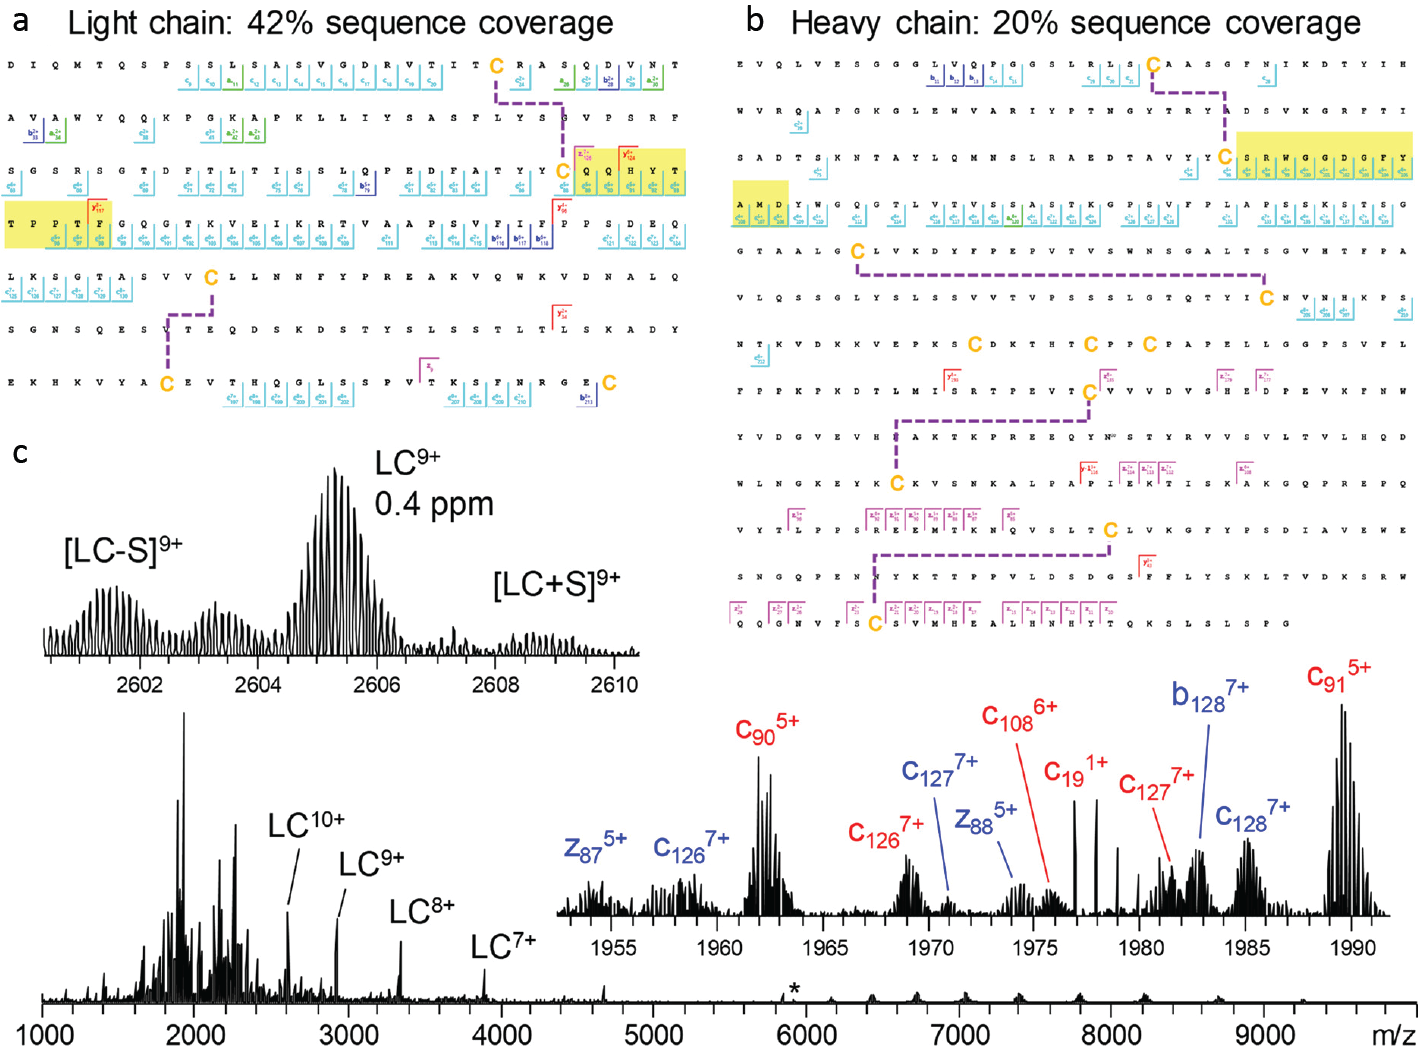
\includegraphics[]{Chapter.1/Figures/f5.png}
  \caption{
    \textbf{Light chain ~~a) and glycosylated heavy chain ~~b) fragmentation maps illustrate sequence coverage produced by the combination of ECD and HCD on Trastuzumab.} Disulphide bonds are shown by dashed lines, CDR3 regions are highlighted in yellow. The corresponding fragmentation spectrum ~~c) for the 25+ charge state of intact Trastuzumab with insets displaying the zoomed in region containing the 9+ charge state of the light chain and various fragment ions. Red and blue fragment ion labels correspond to the light and heavy chain, respectively. Asterisk indicates the mass-selected precursor ion. Figure adapted from Shaw et al. \cite{shaw2020direct}
  }
  \label{fig:fig1.5}
\end{figure*}


\subsubsection{Dedicated software solutions for MS-based antibody sequencing}
The various sample preparation methods and intricate experimental designs presented above result in extended datasets that are not feasible for manual interpretation. Thus, development of dedicated software tools for data interpretation is essential.
With regards to BU MS data, presently, two popular software suites are tailored towards \emph{de novo} sequencing of antibodies, SuperNovo \cite{sen2017automated} and PeaksAB \cite{tran2016complete, ma2003peaks:}. These suites can utilize the benefits of data generated by using multiple enzymes, multiple fragmentation methods, and the use of a homologous antibody germline sequence database like IMGT to make a complete \emph{de novo} sequence prediction based on the BU MS data. More specifically, the software iteratively screens predicted peptides against the germline gene segments of the antibody to determine the positions on the final chain construct. Homologous germline sequence candidates represent scaffolds that are then modified to account for the highest scoring predicted peptides. This allows for predicting both heavy and light chain sequences with a minimal error rate of only a few single amino acids per sequenced antibody. A downside, however, is that the software works so far exclusively for sequencing single, highly purified antibodies.
Novel software solutions for \emph{de novo} antibody sequencing are emerging and advancing in parallel with improvements in experimental design and instrumentation. The fast development of new \emph{de novo} sequencing strategies encourages the development of new software solutions and improvement of already established tools and requires adaptable software to accommodate the frequent and considerable shifts in \emph{de novo} sequencing approaches, such as the inclusion of TD or MD MS data, multiple fragmentation methods or the analysis of polyclonal samples as opposed to mAbs.

\subsubsection{Combining peptide- and protein-centric MS approaches for antibody sequencing}
Recent advances in protein-centric MS have spawned various software tools that use these data either in a standalone manner, such as in Twister \cite{vyatkina2015de, vyatkina2017de}, or integrate them with BU MS data, as in TBNovo \cite{liu2014de}. Twister applies methods similar to those used for BU MS sequencing, recombining individual sequence tags (rather than peptide reads) into longer sequences using a specific implementation of de Bruijn graphs (T-Bruijn graphs) and sequence tag convolution \cite{vyatkina2015de, vyatkina2017de}. TBNovo uses sequence tags and precursor masses from TD MS to provide a scaffold for positioning the \emph{de novo} predicted peptide reads to fill the complete sequence. Their analysis makes use of external BU \emph{de novo} sequencing software, PEAKS \cite{ma2003peaks:}, and was tested on protein mixtures. TBNovo has not achieved widespread adoption, perhaps due to the software’s complexity and because protein-centric MS was still barely practiced at the time of its first release.
Although antibody sequencing at the protein level is still not trivial, it is being applied on a steadily increasing scale in academia and industry. Efforts to extend the sequencing of antibodies to polyclonal mixtures have however proven extremely challenging. The first obstacle is sample availability. While recombinant mAb samples are typically available in milligram quantities, polyclonal antibody samples are often derived from clinical samples and thus will only be available in limited quantities. Because the median concentration of individual clones in plasma is $\sim$1 µg/mL the available protein per individual clone is generally orders of magnitude less compared to mAbs \cite{bondt2021human}. Furthermore, isolation of individual clones is extremely challenging, further complicating the sequencing process as most software tools are exclusively designed for assembling a single antibody and therefore fail when data represents several alike Ig sequences. Additionally, in complex endogenous polyclonal antibody mixtures, key sequence evidence on the hypervariable regions is often not detected due to a dilution effect, whereby sequence information from the conserved regions becomes amplified (as the latter is present in every clone) and thus suppresses the signal of the CDRs, which are unique for all clones. Even though the algorithms developed for mAb sequencing are not directly applicable for polyclonal antibody sequencing, they provide a great starting point for developing new tools.

\subsection{Hybrid and multi-omics approaches for studying antibody repertoires}
One way to further bridge the gap between sequencing of a single purified antibody and those present in bodily fluids, e.g., serum, is to use hybrid or multi-omics strategies. Using a multi-omics approach, for instance, by supplementing BU MS data with genomics or transcriptomics data derived from the same donor, allows bypassing some challenging aspects of genuine \emph{de novo} sequencing, albeit at the cost of a more complex, labour- and data-intensive workflow (\textbf{\autoref{fig:fig1.2}c}). Presently, direct \emph{de novo} sequencing of antibodies from a complex mixture is still a tremendous challenge. However, integrating complementary information from multiple sources makes it possible to derive valuable data, even on endogenous antibody repertoires. Several approaches have been pioneered recently, as depicted in \textbf{\autoref{fig:fig1.6}} and described in more detail below.

\subsubsection{Ig-seq}
Since the CDRs of the antibodies largely determine antigen specificity, it comes as no surprise that methods specifically targeting CDR-derived peptides have emerged. Notably, the Ig-seq method pioneered by Lavinder et al. \cite{lavinder2015next-generation} in the Georgiou lab applies B-cell sequencing of a given donor to construct a database of putative CDR3 heavy chain peptides. This database is then used to identify and quantify antibodies using CDR-specific tryptic peptides, effectively side-stepping the need for complete \emph{de novo} sequencing (\textbf{\autoref{fig:fig1.6}a}). This workflow is very effective because trypsin-targeted residues (arginine and lysine) are found to precede the CDR3 specifically and are found in the relatively conserved FR4 of the heavy chain, ensuring that tryptic peptides contain the heavy chain CDR3 in the majority (>92\%) of IgG clones \cite{lavinder2014identification}. BU MS is highly optimized for measuring and detecting tryptic peptides, which makes this approach highly effective, as shown when this method was applied to the longitudinal monitoring of influenza antibodies over multiple years. Monitoring the effects of influenza vaccinations showed that $\sim$60\% of the response to vaccination originated from pre-existing clonotypes and highlighted the existence and relatively high abundance of broadly protective, non-neutralizing antibodies \cite{lee2016molecular-level}. Years later, follow-up studies showed that persistent antibodies account for >70\% of the serum response over five years, further promoting the efficiency and strength of the Ig-seq method \cite{lee2019persistent}. It should be noted that relying solely on sequences obtained from PBMCs may provide an incomplete database \cite{guthals2017de}, as it is only feasible to obtain a subset of PBMCs for analysis. Nonetheless, Ig-seq presents one of the most efficient and successful approaches to analyse and identify clones in Ig repertoires and monitor how they (dis)appear following a change in physiology, e.g., infection or vaccination.
\begin{figure*}[!htb]
  \center
  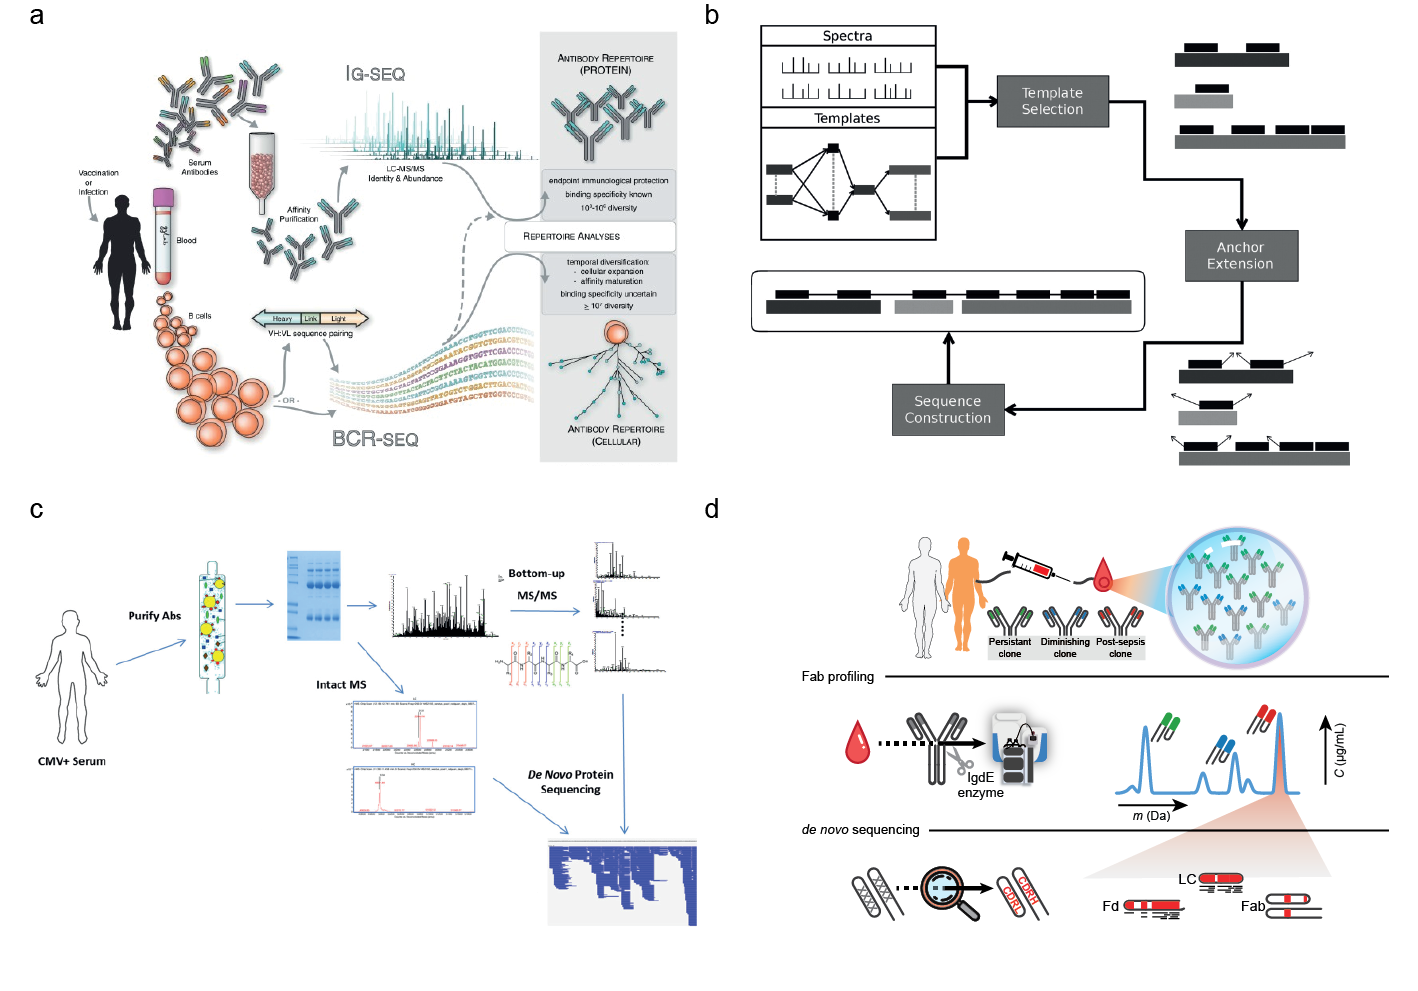
\includegraphics[]{Chapter.1/Figures/f6.png}
  \caption{
    \textbf{Selected recent approaches aiming towards MS-based \emph{de novo} sequencing of serum antibodies.} ~~a) In Ig-seq \cite{lavinder2015next-generation} a personalized database generated by BCR sequences is used to identify specific clones, using tryptic peptides covering the CDR3 region. Figure adapted from Lavinder et al. \cite{lavinder2015next-generation} ~~b) Template proteogenomics \cite{castellana2010template} use genomic data to generate template sequences. The specific construction of the templates can be defined by the user from either whole genome sequencing or BCR sequencing data. Figure adapted from Castellana et al. \cite{castellana2010template} ~~c) PolyExtend \cite{guthals2017de} helped to analyse a polyclonal mixture of antigen-specific purified antibodies measured by BU MS and intact mass measurements. Using a user-assisted algorithm, these data from different MS modalities were combined to sequence the most abundant clones. Figure adapted from Guthals et al. \cite{guthals2017de} ~~d) Fab profiling \cite{bondt2021human} measures and quantifies intact masses of Fabs to provide a view of the IgG1 clonal repertoire, enabling to quantify and monitor individual clones. Abundant serum clones are identified by using BU and MD MS data iteratively to generate full IgG \emph{de novo} sequences. Figure adapted from Bondt et al. \cite{bondt2021human}
  }
  \label{fig:fig1.6}
\end{figure*}


\subsubsection{Alternative proteogenomics approaches}
Extending beyond the Ig-seq strategy, proteogenomics approaches as taken by Castellana et al. \cite{castellana2010template} incorporate personalized genomics data into the antibody sequencing workflow to identify complete antibody sequences. In their software package GenoMS \cite{castellana2010template} they accept both proteomic and genomic databases as input, which are used to reconstruct antibody (sub)sequences from BU MS data. The database is used to find a homologous template sequence, whereby missing, mutated, and spliced genes are considered. The software also allows for a high degree of flexibility through user-defined constraints. In addition, users can define how the template database is used, excluding certain genes, or using multiple gene segments (V, D, J, or C) to make up a single sequence (\textbf{\autoref{fig:fig1.6}b}). As often occurs with hybrid approaches, the power of this proteogenomics strategy comes at a cost. While broadly applicable and very powerful, the required expertise increases because of the use and combination of multiple omics techniques. However, when successfully applied, this workflow produces exciting results, as recently shown in the analyses of antibodies from immunized rabbits \cite{bonissone2020serum} and the characterization of neutralizing antibodies against the Ebola virus antigen \cite{gilchuk2021proteo-genomic} with notable improvements in integration and visualization of the data. Unfortunately, not all these tools are currently publicly available, although several underlying protocols are open source \cite{cha2017antibody, safonova2015igrepertoireconstructor:, bonissone2016immunoglobulin}.

\subsection{Protein-centric sequencing of endogenous antibodies}
Some attempts have emerged aiming at novel antibody discovery by MS-based sequencing alone, directly from serum samples or other liquid biopsies, circumventing the need for genomics/transcriptomics data (multi-omics approaches). Above we reviewed several techniques for sequencing purified antibodies. As we pointed out, these methods are geared towards highly purified mAb samples and are therefore not directly applicable for polyclonal antibody mixtures. However, advancements in sample preparation, instrumentation, and bioinformatics make it possible to obtain partial and sometimes complete \emph{de novo} sequences of endogenous antibody clones by combining different mass spectrometric techniques, as discussed further below.

\subsubsection{Antigen-specific capture}
For many pathologies, it is common to screen patient’s serum for antibodies that exhibit activity against the antigens originating from the pathogen, for example, by enzyme-linked immunosorbent assay (ELISA). Using pathogen-based antigens, it is also possible to capture specific antibody clones from serum that exhibit high affinity against the antigen. This typically reduces the complexity of the antibody mixture substantially. Nevertheless, it is still nearly impossible to reduce the complexity down to a single clone, as often, multiple antibodies with varying affinities for any given antigen co-occur. An example of a capturing method whereby additional intact mass data was used to derive \emph{de novo} sequences was described by Guthals et al. \cite{guthals2017de}. Following affinity purification of antibodies from the serum of a cytomegalovirus-exposed individual, using the glycoprotein B antigen, both intact mass and BU MS measurements were performed. Their semi-automated software PolyExtend seeks to use the intact mass measurements to retrieve the average mass of the most abundant species in an antibody mixture, which in turn is used as a mass constraint for a sequence derived using the BU MS data (\textbf{\autoref{fig:fig1.6}c}). PolyExtend builds further upon the meta-SPS algorithm \cite{guthals2012shotgun}, which was initially designed to extend subsequences by assembling multiple sequence predictions into longer subsequences. However, diverging extensions for the same subsequence are treated as sequencing errors with one extension selected for the output. In the case of antibodies, such divergences may indicate the presence of two similar clones. To account for this, the software displays the possible extensions as a ranked list, and the user can then select the extension. This approach aims at expanding the \emph{de novo} sequencing capabilities of the previously established meta-SPS algorithm to deal with simultaneous presence of multiple clones, and Guthals et al. \cite{guthals2017de} demonstrated a clear proof of concept.

\subsubsection{Antibody profiling and sequencing in polyclonal mixtures}
While it is still not possible to \emph{de novo} sequence entire serum antibody repertoires, recent advances in LC-MS of intact proteins enabled detecting and resolving single clones from complex antibody mixtures.
For instance, developments have been made that specifically profile intact light chains from serum, even providing partial sequence information by using MD MS. Impressively these studies successfully demonstrate the analysis in serum without requiring antigen-specific capture, although they used either a spiked-in mAb as a model or worked with disease models that cause monoclonal Ig overexpression in serum (mono-gammopathy) such as multiple myeloma. Nonetheless, these studies demonstrated that detection and characterization of individual endogenous light chains is possible \cite{he2017analysis, he2019classification, mills2015detecting, sharpley2019novel, dupré2021de}. Taking this one step further, Wang et al. \cite{wang2019top-down} developed a method to detect individual Fab fragments in serum. They were able to identify tens of heavy and light chains of serum autoantibodies. Although attempts were made to \emph{de novo} sequence these antibodies at the intact protein level, the obtained results were limited to a few sequence tags. In light of the SARS-CoV-2 pandemic, Melani et al. \cite{melani2022next-generation} focused their profiling efforts on the vaccine-targeted spike protein receptor-binding domain. The approach is named Ig-MS and features two novel metrics for capturing the intensity and complexity of the antibody response. In short, the method uses affinity purification to capture antigen-specific clones. A mAb-containing standard is spiked in for quantitation, and the sample is disulphide-reduced. After reduction, individual ion MS \cite{kafader2020multiplexed} is used to measure a mass fingerprint of the sample. The ratio between the intensity of clonal peaks and the standard is used to estimate the response (“Ion Titer”), and the complexity of the response (“Degree of Clonality’) is assessed by the ratio of the most intense light chain peak to that of the summed intensity of all light chain peaks. Finally, these metrics are correlated to the ELISA-based antibody titer and neutralization efficiency, to verify their accuracy.
In a recent study, Bondt et al. \cite{bondt2021human} used an approach to generate Fab fragments exclusively from the entire IgG1 repertoire. They were able to longitudinally profile IgG1 Fabs from the serum of both healthy and sepsis-inflicted donors without the need for any enrichment of specific clones. They observed a range of 50-500 distinct detectable IgG1 Fab clones per donor and showed that most clones persist over multiple months of sampling. Contrary to widely held belief, they showed that the IgG1 repertoire is in abundance dominated by just a few hundred clones and that each donor exhibits a unique repertoire of clones. They also managed to directly \emph{de novo} sequence a single highly abundant clone in one of the donors without the aid of antigen-specific capture. The \emph{de novo} sequencing was achieved by a combination of protein-centric sequencing using ETD, and a BU MS approach using multiple proteases for digestion. First, closely matching light and heavy chain germline templates were selected from the IMGT database. Subsequently, the data was used to refine these templates iteratively, yielding the final mature sequence. This provided proof of concept that \emph{de novo} sequencing of clones directly from serum is feasible, although still arduous and limited to specific cases (\textbf{\autoref{fig:fig1.6}d}). Notably, the determined sequences contained more mutations (compared to germline sequences) than expected from the reported rates from BCR sequencing studies \cite{kitaura2017different}, which is indicative of potential discrepancies between protein-level and gene-level sequencing. This first attempt focused exclusively on IgG1, by using an IgG1-specific protease to generate the Fab fragments. In another work, Bondt et al. \cite{bondt2021direct} extended their method to IgA1 by using a protease specific to the O-glycans present in IgA1 hinge region to generate Fab fragments, albeit now exclusively from IgA1. Overall, they showed that – similar to serum IgG1 – just a handful of clones dominates the secretory IgA1 profile of human milk.
Using a somewhat comparable approach, Dupré et al. \cite{dupré2021de} analysed isolated light chains from the urine of a patient affected by multiple myeloma. They assembled \emph{de novo} data from peptides into a full-length sequence, using the intact mass data as a scaffold. Subsequently, they used TD MS to validate their findings and further characterize the proteoforms of the light chains, including PTMs. The BU MS data further supported the resulting proteoforms, showing a similar added benefit from iteratively combining BU and TD MS data.

\subsection{Additional benefits of studying antibodies at the protein level}
The capabilities of MS allow for antibody characterization beyond the primary amino acid sequence. Antibodies are known to harbour multiple important PTMs: Fab- and Fc-glycosylation \cite{haan2020monitoring}, deamidation \cite{yan2018structure}, and C-terminal truncation \cite{beyer2018microheterogeneity}, to name a few. Moreover, although the disulphide bonds in IgG1 are thoroughly described, other subclasses, notably IgG2, appear to occur as structural isomers induced by different disulphide-bridge patterns. These PTMs and disulphide bridges become even more pronounced in IgA and IgM, which can form higher-order structures connected by the joining-chain in serum and other bodily fluids. All these features influence the antibody’s efficacy and stability. Such information cannot easily be obtained at the nucleotide level, requiring protein-level analysis.
\clearpage

\section{Thesis overview}
Throughout this thesis, I detail my efforts to develop computational workflows and tools that facilitate the analysis of complex LC-MS proteomics data. There is a strong focus on the analysis of antibody repertoires, apart from Chapter 2 which focuses on analyzing cross-linking MS data. The work described in this chapter shaped what became the guiding principle of my academic efforts; that \emph{standardized computational tools are of vital importance for reproducible research}. As such, I consider it the spiritual predecessor to the subsequent chapters and an important example of the central theme.
\bigskip\\
\textbf{Chapter 2} describes how we developed CrossID, a tool to analyze large and complex cross-linking proteomic datasets. CrossID was developed to facilitate explorative analysis of large amounts of crosslinking data. We show that integration of data from multiple sources can provide valuable insights, as the integrated data from protein databases enables gene ontology enrichment analysis and grouping based on function. Furthermore, we showcase how mapping of crosslinked residues onto 3D-structural models for proteins can help refine these models or help to generate models for protein complexes.
\bigskip\\
In \textbf{Chapter 3}, the LC-MS based antibody repertoire profiling approach which enabled the research in \textbf{Chapter 4} and \textbf{5} is introduced. In this initial application of the technique on a cohort of sepsis patients we found the serological IgG1 repertoires to be unique to each individual, stable over time, responsive to physiological events and relatively simple, consisting of several hundred clones despite there being an enormous number of theoretically possible clones. Furthermore, this chapter provides proof of concept for \emph{de novo} sequencing of endogenous antibodies by using a multi-tier mass spectrometry approach to sequence the most abundant clone for a donor.
\bigskip\\
\textbf{Chapter 4} describes the analysis of breastmilk SIgA1 profiles of six mothers who had received two identical SARS-CoV-2 vaccinations over 16 timepoints. We use the extensive sampling and repeated vaccination to define clonal populations based on the detection window of these clones relative to the vaccination events. We also discover that the second vaccination induces the emergence of a population of novel clones and show that titer fluctuations as measured by ELISA can be driven by highly divergent clonal populations.
\bigskip\\
In \textbf{Chapter 5}, we build upon the proof of concept for \emph{de novo} sequencing of endogenous antibodies by hybrid top-down and bottom-up mass spectrometry approaches. We present a more standardized workflow for sequencing antibody chains in mixtures. Our approach resolves ambiguity in sequence predictions for the hypervariable complementarity determining regions by mass-filtering candidate sequences based on the gap size between adjacent framework regions, which we determine using middle-down fragmentation data.
\bigskip\\
Finally, \textbf{Chapter 6} contains a summary and a discussion of the advances that enabled the work in this thesis, the impact of the findings for others in the field, the challenges that lay ahead and how they may be overcome, along with an outlook on where I believe the field is heading.
\newpage
\section*{References}
\bibliographystyle{Stylesettings/pnas}
\patchcmd{\thebibliography}
{\clubpenalty 4000\widowpenalty 4000}
{\clubpenalties 1 10000 \widowpenalties 1 10000}
{}{}
\bibliography{chapmerge}
\stopthumb


%%refs (does not alter the tex cause commented, just for retrieval)
%% \cite{georgiou2014promise}
